\section{Imagen}

Imagen \cite{imagen} is a text-to-image diffusion model that builds on the power of large transformer language models \cite{transformer} to generate high-fidelity images. The combination of diffusion (section \ref{sec:diff}) and LLMs have shown remarkable outputs. One of the main observation in the paper that the researchers discovered is that a large frozen LLM has bigger impact on the fidelity of generated images than increasing the amount of parameters in the image diffusion model. Another contribution in the paper is the introduction of new benchmark to evaluate text-to-image models such as DALL-E \cite{dalle}, VQ-GAN+CLIP \cite{vqgan_clip}, latent diffusion models \cite{stable_diffusion}, GLIDE \cite{glide}, and DALLE-E 2 \cite{dalle_2}.










\subsection{Text-to-Text Transfer Transformer (T5)}

\textbf{T}ext-\textbf{t}o-\textbf{T}ext \textbf{T}ransfer \textbf{T}ransformer (T5) \cite{t5_model} is a model that was introduced by Google Research that treats tasks as a text-to-text problems. For example, for summorization tasks we could prompt the LLM: "Please summorize the following: ...", for translation tasks we could prompt the LLM: "Translate from English to French the word 'You'", as well as for text classification, question answering, conversations, and other tasks. In short, this knowledge can be viewed as developing a 'general-purpose' model that can understand text.  Instead of explicitly training the model to learn words or text, such as in the case of \textbf{word vectors} \cite{cbow_word2vec}, a more common practice is to \textbf{pre-train} \cite{bert} the model on data-rich task in an unsupervised manner. The model T5 is open-source and was trained on large corpura of textual data. The base version of the model (T5-base) consists of 220 million parameters, while the largest version of the model (T5-XXL) consists of 11 billion parameters. In the context of Imagen, the Imagen model uses a frozen version of T5-XXL model to encode conditional text prompts.

This pre-training approach causes the model to develop general-purpose abilities that are then used in downstream tasks (translation, summorization, conversation and more). Unsupervised pre-training is appealing because unlabeled text data is abundant and available on the Internet. For example, the Common Crawl project \cite{common_crawl_project} is a non-profit organization that crawls the internet and provides free access to its achived datasets to the publlic. A lot of research has been done on the training of models on large scale dataset, and the consensus is that the larger the dataset, the better the model performs \cite{radford2019language} \cite{jozefowicz2016exploring} \cite{hestness2017deep}. The T5 models were trained on the "Colossal Clean Crawled Corpus" (C4) dataset, which consists of 750GB of English text data scraped from the web.

The architecture of T5 consists of an encoder-decoder transformer model, closly follows the implementation in the paper that introduced the transformer model \cite{transformer}. It first maps an input token sequence to embeddings, which are passed to the encoder. The encoder consists of stacked blocks, each with a \textbf{self-attention layer} (section \ref{subsec:cross_attention}) followed by a feed-forward network (simple fully connected layer). Layer normalization (appendix \ref{appendix:layer_normalization}) is applied before each component, using a simplified version without additive bias \footnote{Layer normalization rescales and shifts the activations of a layer by rescaling values (e.g. between 0 and 1) and by additive bias. Removing the additive bias means the model won't apply the extra shift; it only rescales the activations without any other adjustments.}. Residual connections and dropout are applied throughout. The decoder mirrors the encoder but includes an additional attention layer to attend to encoder outputs and uses autoregressive self-attention to focus on past outputs. The final decoder output passes through a dense layer with shared weights from the input embeddings. 

\textbf{The training objective} of T5 model is called \textbf{span corruption}, which is stronger version of \textbf{masked language modeling}. Given a sentence, some words and some contigous words are masked (in masked language modeling, only single words are masked), and the model should predict those words. For example: "Thank you for inviting me to your party last week", where the masked words are "for inviting" and "last". And the model should predict those words in the following sentence: "Thank you [MASKED] me to your party [MASKED] week". The model should learn to reconstruct the missing text. The actual loss function is to choose the correct words by similarity in the embeddings space, which is where cross-entropy is commonly used for.

\begin{figure}[h]
    \centering
    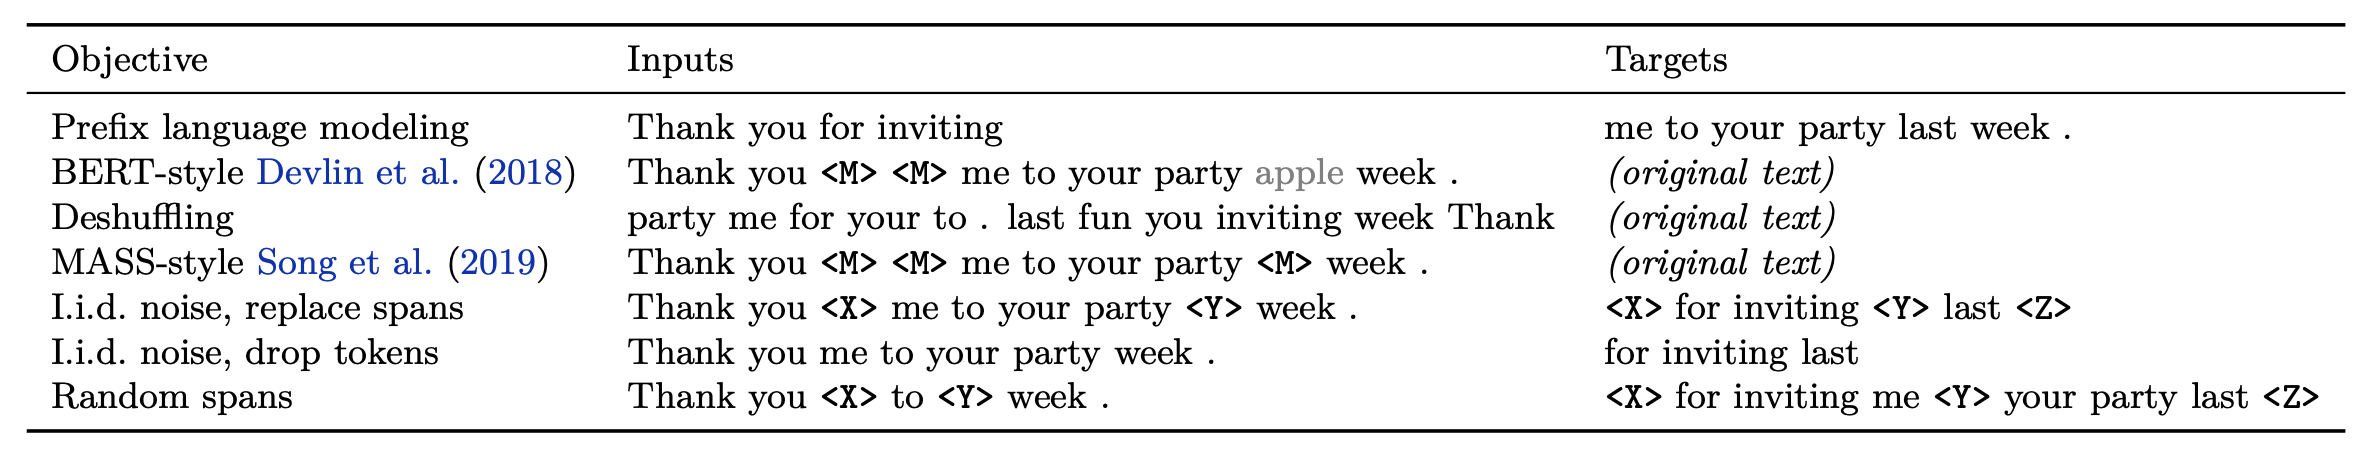
\includegraphics[width=1\textwidth]{images/imagen/t5_objectives.png}
    \caption{The unsupervised training objectives of T5 model. \textless M\textgreater\ denotes shared mask token (the same mask token is used to represent all masked positions in the input). \textless X\textgreater, \textless Y\textgreater, and \textless Z\textgreater\ denote sentiel tokens (with unique token IDs, they mark specific masked positions that the model should reconstruct).}
\end{figure}







\subsection{Architecture}

The architecture of Imagen consists of T5-XXL (T5-Extra Extra Large) text encoder. This model consists of 11 billion parametersand requires significant computational resources to train and fine-tune.

The T5-XXL model is the largest version of the T5 model.


\begin{figure}
    \centering
    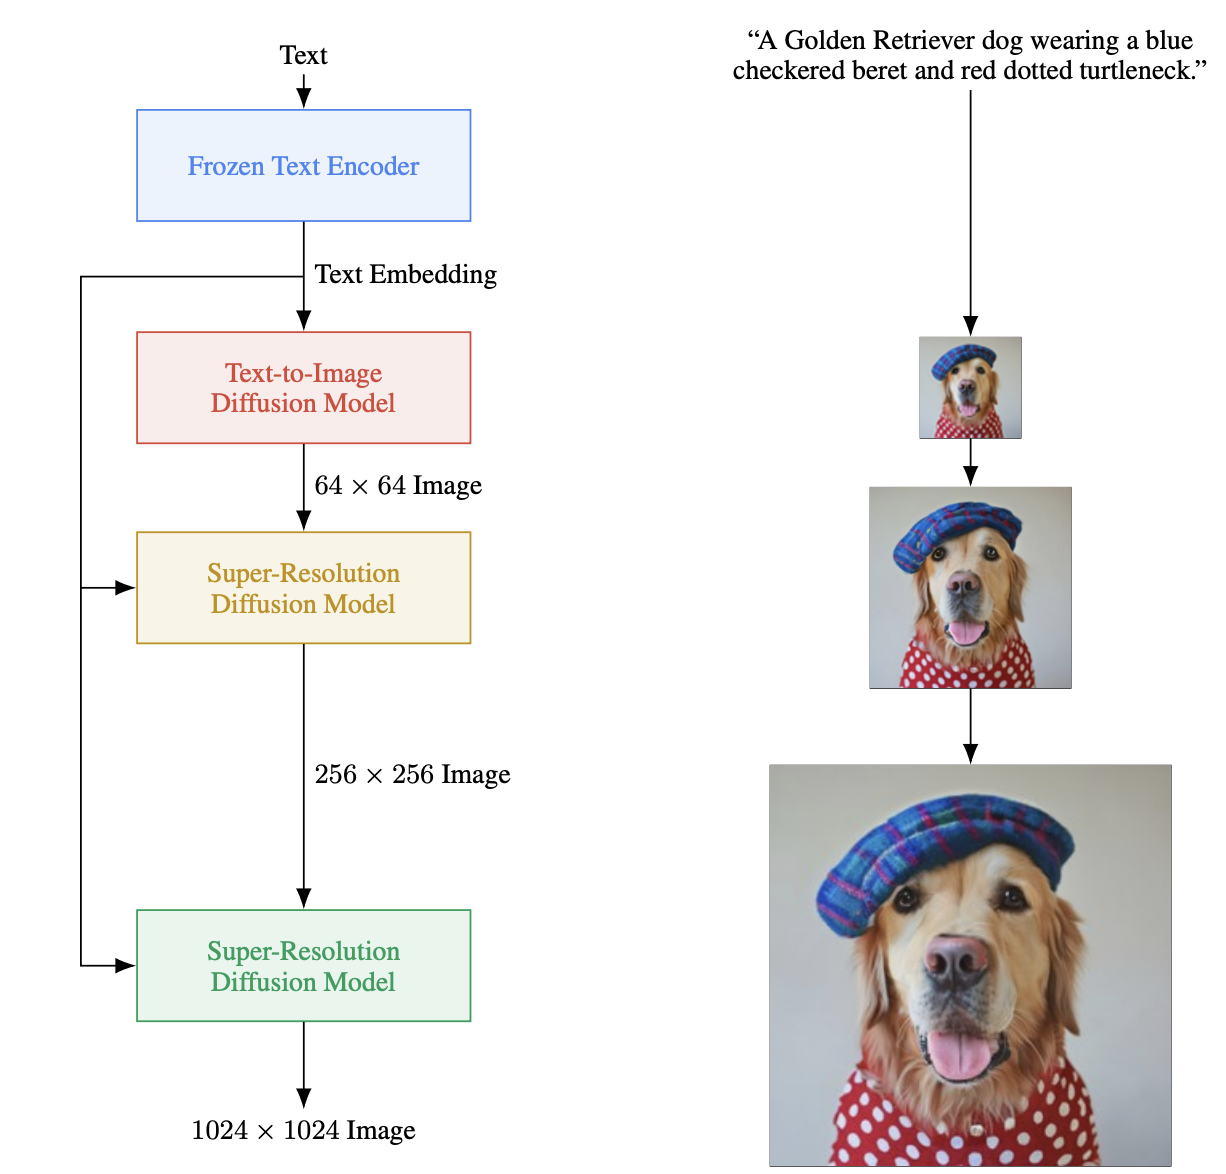
\includegraphics[width=0.5\textwidth]{images/imagen/architecture.png}
    \caption{Imagen architecture.}
    \label{fig:imagen_architecture}
\end{figure}